
\documentclass[preprint,12pt]{elsarticle}


\usepackage[spanish]{babel}
\usepackage{amssymb}
\usepackage{graphicx}
\usepackage{lineno}
\usepackage[utf8]{inputenc}
\usepackage{url}




\journal{Journal Name}

\begin{document}
	
	
	\newpage
	
	\subsection{Ejemplos \\}
		
		\begin{enumerate}[A)]
			\item BIG DATA 
			
			\begin{figure}[htb]
				\begin{center}
					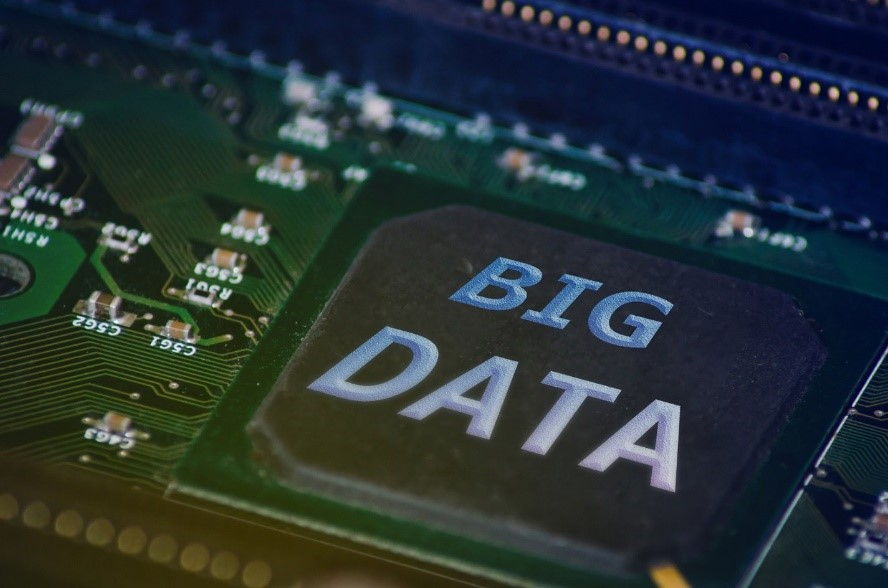
\includegraphics[width=8.5cm]{./Imagenes/img1}
				\end{center}
			\end{figure}
		
			Big Data es un término que describe el gran volumen de datos, tanto estructurados como no estructurados, que inundan los negocios cada día. Pero no es la cantidad de datos lo que es importante. Lo que importa con el Big Data es lo que las organizaciones hacen con los datos. Big Data se puede analizar para obtener ideas que conduzcan a mejores decisiones y movimientos de negocios estratégicos.\cite{bib03:BA:Online} \\ 
			
			¿Porque es tan importarnte este concepto?\\
			
			Lo que hace que Big Data sea tan útil para muchas empresas es el hecho de que proporciona respuestas a muchas preguntas que las empresas ni siquiera sabían que tenían. En otras palabras, proporciona un punto de referencia. Con una cantidad tan grande de información, los datos pueden ser moldeados o probados de cualquier manera que la empresa considere adecuada. Al hacerlo, las organizaciones son capaces de identificar los problemas de una forma más comprensible.\\
			
			La recopilación de grandes cantidades de datos y la búsqueda de tendencias dentro de los datos permiten que las empresas se muevan mucho más rápidamente, sin problemas y de manera eficiente. También les permite eliminar las áreas problemáticas antes de que los problemas acaben con sus beneficios o su reputación.\\
			
			El análisis de Big Data ayuda a las organizaciones a aprovechar sus datos y utilizarlos para identificar nuevas oportunidades. Eso, a su vez, conduce a movimientos de negocios más inteligentes, operaciones más eficientes, mayores ganancias y clientes más felices. Las empresas con más éxito con Big Data consiguen valor de las siguientes formas:\\
			
			\textbf{Reducción de coste}. Las grandes tecnologías de datos, como Hadoop y el análisis basado en la nube, aportan importantes ventajas en términos de costes cuando se trata de almacenar grandes cantidades de datos, además de identificar maneras más eficientes de hacer negocios.\\
			
			\textbf{Más rápido, mejor toma de decisiones.} Con la velocidad de Hadoop y la analítica en memoria, combinada con la capacidad de analizar nuevas fuentes de datos, las empresas pueden analizar la información inmediatamente y tomar decisiones basadas en lo que han aprendido.\\
			
			\textbf{Nuevos productos y servicios.} Con la capacidad de medir las necesidades de los clientes y la satisfacción a través de análisis viene el poder de dar a los clientes lo que quieren. Con la analítica de Big Data, más empresas están creando nuevos productos para satisfacer las necesidades de los clientes.\\
			
							
			\item MACHINE LEARNING 
			
			\begin{figure}[htb]
				\begin{center}
					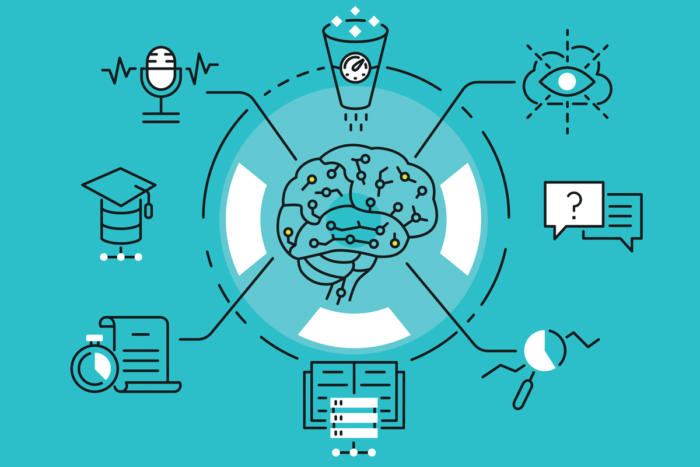
\includegraphics[width=8.41cm]{./Imagenes/img2}
				\end{center}
			\end{figure}
		
			Machine Learning es una disciplina científica del ámbito de la Inteligencia Artificial que crea sistemas que aprenden automáticamente. Aprender en este contexto quiere decir identificar patrones complejos en millones de datos. La máquina que realmente aprende es un algoritmo que revisa los datos y es capaz de predecir comportamientos futuros. Automáticamente, también en este contexto, implica que estos sistemas se mejoran de forma autónoma con el tiempo, sin intervención humana.\cite{bib01:BA:Online} \\
			
			
			El campo de aplicación práctica depende de la imaginación y de los datos que estén disponibles en la empresa. Estos son algunos ejemplos:
			\begin{itemize}
				\item Detectar fraude en transacciones.
				\item Predecir de fallos en equipos tecnológicos.
				\item Prever qué empleados serán más rentables el año que viene (el sector de los Recursos Humanos está apostando seriamente por el Machine Learning).
				\item Seleccionar clientes potenciales basándose en comportamientos en las redes sociales, interacciones en la web…
				\item Predecir el tráfico urbano.
				\item Saber cuál es el mejor momento para publicar tuits, actualizaciones de Facebook o enviar las newsletter.
				\item Hacer prediagnósticos médicos basados en síntomas del paciente.
				\item Cambiar el comportamiento de una app móvil para adaptarse a las costumbres y necesidades de cada usuario.
				\item Detectar intrusiones en una red de comunicaciones de datos.
				\item Decidir cuál es la mejor hora para llamar a un cliente.
				
			\end{itemize}
		
			La tecnología está ahí. Los datos también. ¿Por qué esperar a probar algo que puede suponer una puerta abierta a nuevas formas de tomar decisiones basadas en datos? Seguro que has oído que los datos son el petróleo del futuro. Ahora ya puedes empezar a bombearlo
							
		\end{enumerate}
	
	\newpage
	
	\section{Bussines Intelligence}
	\label{S:2}
	
	BI es un conjunto de técnicas que tienen por finalidad transformar los datos de una empresa en información, identificando posibles indicadores y que estos puedan ser explotados(por ejemplo en cubos), ayudando a la mejora en la toma de decisiones.\\
	
	Nota: Es común confundir que BI solo consiste en la generación cubos, pero ésta es tan solo una parte de toda la arquitectura de BI como se muestra en la figura:
	\begin{figure}[htb]
		\begin{center}
			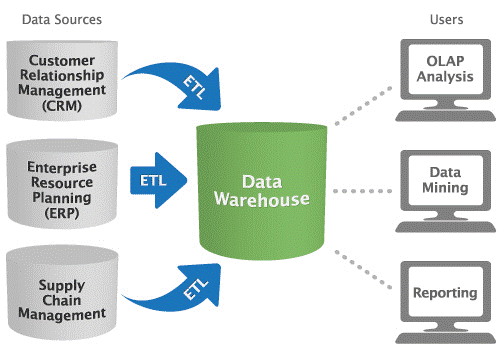
\includegraphics[width=9.5cm]{./Imagenes/img3}
		\end{center}
	\end{figure}
	
	Hasta ahora vamos bien, pero y ¿Qué es Business Analytics?. BA también es un conjunto de técnicas (algoritmos predictivos y modelos estadísticos), pero a diferencia de BI éstas nos permiten predecir posibles resultados (en un futuro), es aquí donde aparecen términos como:Machine Learning, Data Mining, etc.\\
	
	BI nos ayuda a responder preguntas como ¿Quién? ¿Cuándo paso? ¿Qué pasó?, mientras que BA nos ayuda a responder preguntas como ¿Cuándo volverá a suceder?  ¿Quiénes podrían volver a hacerlo?\\
	
	BI se enfoca en toda la data histórica hasta el presente, mostrándote por ejemplo en una empresa como han ido variando sus ventas a lo largo del o de los años, mientras que BA nos permitiría predecir en que mes(futuro) podríamos tener más ventas, teniendo como base los datos históricos que se obtuvieron de BI, es por eso que se puede concluir que estas dos técnicas no son ajenas la una de la otra, sino mas bien son complementarias.\cite{bib01:BI:Online}
		
\end{document}

%%
%% End of file `elsarticle-template-1-num.tex'.
